%\documentclass[landscape,a0b,final,a4resizeable]{a0poster}
%\documentclass[portrait,a0b,final]{a0poster}
\documentclass[a1,portrait,final]{a0poster}
%\documentclass[final]{beamer}
%\mode<presentation>
%{
%\usepackage[orientation=landscape,size=a0,scale=1.4,debug]{beamerposter}
%\documentclass[portrait,a0b,final,a4resizeable]{a0poster}
%\documentclass[portrait,a0b,final]{a0poster}
%%% Option "a4resizeable" makes it possible ot resize the
%   poster by the command: psresize -pa4 poster.ps poster-a4.ps
%   For final printing, please remove option "a4resizeable" !!

\usepackage[ruled,lined]{algorithm2e}
\def\algorithmautorefname{Algorithm}
\SetKwIF{If}{ElseIf}{Else}{if}{then}{else if}{else}{endif}
\usepackage{npbayes}
\usepackage[usenames,dvipsnames]{xcolor}
\usepackage{tkz-berge}
\usetikzlibrary{fit,shapes}
\usepackage{amsmath,amssymb,rotating,multirow}
\usepackage{calc}
%%
%% The tikz package is used for doing the actual drawing.
\usepackage{tikz}
%%
%% In order to be able to put arrowheads in the middle of directed edges, we need an extra library.
\usetikzlibrary{decorations.markings}
%%
%% The next line says how the "vertex" style of nodes should look: drawn as small circles.
\tikzstyle{vertex}=[circle, draw, inner sep=0pt, minimum size=6pt]
%%
%% Next, we make a \vertex command as a shorthand in place of \node[vertex} to get that style.
\newcommand{\vertex}{\node[vertex]}
%%
%% Finally, we declare a "counter", which is what LaTeX calls an integer variable, for use in
%% the calculations of angles for evenly spacing vertices in circular arrangements.
\newcounter{Angle}

\renewcommand{\baselinestretch}{0.97}
\usepackage[usenames,dvipsnames]{xcolor}
\thispagestyle{empty}

\usepackage{epsfig,bm}
\usepackage{multicol}
\usepackage{pstricks,pst-grad}
\usepackage{amssymb,amsmath,amstext,graphicx,amsopn,amsfonts,bm,amsthm}
\newcommand{\draw}{\stackrel{\text{draw}}{\sim}}

\RequirePackage[colorlinks,citecolor=blue,urlcolor=blue]{hyperref}
 

%\usepackage[sort&compress,numbers]{natbib}
%\bibpunct{(}{)}{;}{a}{}{,}
%\newtheorem{theorem}{Theorem}
%%%%%%%%%%%%%%%%%%%%%%%%%%%%%%%%%%%%%%%%%%%
% Definition of some variables and colors
%\renewcommand{\rho}{\varrho}
%\renewcommand{\phi}{\varphi}
\setlength{\columnsep}{3cm}
\setlength{\columnseprule}{2mm}
\setlength{\parindent}{0.0cm}

%\newcommand{\indep}{\stackrel{\text{indep}}{\sim}}
\newcommand{\cas}{\buildrel \textrm{\scriptsize a.s.} \over
  \longrightarrow}
\newcommand{\cd}{\buildrel d \over \longrightarrow}
\newcommand{\cp}{\buildrel P \over \longrightarrow}
\newcommand{\R}{\mathbb{R}}
\newcommand{\hatbb}{\boldsymbol{\hat{b}}}
\newcommand{\hatbB}{\boldsymbol{\hat{B}}}
\newcommand{\hatbd}{\boldsymbol{\hat{d}}}
\newcommand{\commentt}[1]{}
\newcommand{\myvfil}[1]{\vskip 0pt plus #1fill}
% \renewcommand{\upsilon}{v}
\newcommand{\lik}{\ell_y(\theta)}
\newcommand{\likil}{\ell_y(\theta_i^{(l)})}
\newcommand{\hd}{\hfill$\diamondsuit$}
\newcommand{\aaa}{\epsilon}
\newcommand{\lt}{\left}
\newcommand{\rt}{\right}
\newcommand{\mbi}{\max_{1 \leq i \leq m} \bxi'\bb}
\newcommand{\bs}{B_{i*}}
\newcommand{\bi}{B_{i}}
\newcommand{\that}        {\mbox{$\hat{\boldsymbol{\theta}}$}}
\newcommand{\utheta}        {\mbox{$\boldsymbol{\theta}$}}
\newcommand{\thhj}{\hat{\theta}_j}
\newcommand{\thhij}{\hat{\theta}_{ij}}
\newcommand{\thiHB}{\hat{\theta}_i^{HB}}
\newcommand{\thih}{\hat{\theta}_i^H}
\newcommand{\thit}{\tilde{\theta}_i^H}


%\renewcommand{\liminf}{\operatornamewithlimits{\textrm{lim\,inf}}}
%\newcommand{\comment}[1]{}
%\newcommand{\bpi}{\boldsymbol{\pi}}
\newcommand{\g}{\,|\,}
\newcommand{\teq}{\!=\!}


%\newcommand{\tr}{\text{tr}}
\newcommand{\btt}{\boldsymbol{\theta}}

\newcommand{\ttt}{\boldsymbol{t}}
\newcommand{\bhat}{\boldsymbol{\hat{\beta}}}
\newcommand{\thb}{\bar{\theta}}
\newcommand{\bx}{\boldsymbol{x}}
\newcommand{\bv}{\boldsymbol{v}}
\newcommand{\bu}{\boldsymbol{u}}
\newcommand{\ur}{\boldsymbol{r}}
\newcommand{\uphi}{\boldsymbol{\phi}}
\newcommand{\uone}{\boldsymbol{1}}
\newcommand{\ue}{\boldsymbol{e}}
\newcommand{\uc}{\boldsymbol{c}}
\newcommand{\bbi}{\boldsymbol{b}_i}
\newcommand{\uw}{\boldsymbol{w}}
\newcommand{\bz}{\boldsymbol{z}}
\newcommand{\be}{\boldsymbol{e}}
\newcommand{\by}{\boldsymbol{y}}
\newcommand{\utt}{\boldsymbol{t}}
\newcommand{\bzero}{\boldsymbol{0}}
\newcommand{\bl}{\boldsymbol{l}}
\newcommand{\util}{\boldsymbol{\tilde{u}}}
\newcommand{\btil}{\boldsymbol{\tilde{\beta}}}
\newcommand{\btils}{\boldsymbol{\tilde{\beta}_*}}
%\newcommand{\bm}{\boldsymbol{m}}
\newcommand{\btilf}{(X'V^{-1}X)^{-1}X'V^{-1}\that}
\newcommand{\btilfs}{(X'V_*^{-1}X)^{-1}X'V_*^{-1}\that}
\newcommand{\bxij}{\boldsymbol{x_{ij}}}
\newcommand{\bxj}{\boldsymbol{x}_j}
\newcommand{\bei}{\boldsymbol{e_{i}}}
\newcommand{\bej}{\boldsymbol{e_{j}}}
\newcommand{\bbary}{\boldsymbol{\bar{y}}}
\newcommand{\thet}{\boldsymbol{\theta}}




%%%%%%%%%%%%%%%%%%%%%%%%%%%%%%%%%%%%%%%%%%%%%%%%%%%%
%%%               Background                     %%%
%%%%%%%%%%%%%%%%%%%%%%%%%%%%%%%%%%%%%%%%%%%%%%%%%%%%

\newcommand{\background}[3]{
  \newrgbcolor{cgradbegin}{#1}
  \newrgbcolor{cgradend}{#2}
   \psframe[fillstyle=gradient,gradend=cgradend,
  gradbegin=cgradbegin,gradmidpoint=#3] (0.,0.,)(1.\textwidth,-1.\textheight)%(-1in,3.5in)(\paperwidth,-\paperheight)
}



%%%%%%%%%%%%%%%%%%%%%%%%%%%%%%%%%%%%%%%%%%%%%%%%%%%%
%%%                Poster                        %%%
%%%%%%%%%%%%%%%%%%%%%%%%%%%%%%%%%%%%%%%%%%%%%%%%%%%%

\newenvironment{poster}{
  \begin{center}
  \begin{minipage}[c]{0.98\textwidth}
}{
  \end{minipage}
  \end{center}
}



%%%%%%%%%%%%%%%%%%%%%%%%%%%%%%%%%%%%%%%%%%%%%%%%%%%%
%%%                pcolumn                       %%%
%%%%%%%%%%%%%%%%%%%%%%%%%%%%%%%%%%%%%%%%%%%%%%%%%%%%

\newenvironment{pcolumn}[1]{
  \begin{minipage}{#1\textwidth}
  \begin{center}
}{
  \end{center}
  \end{minipage}
}



%%%%%%%%%%%%%%%%%%%%%%%%%%%%%%%%%%%%%%%%%%%%%%%%%%%%
%%%                pbox                          %%%
%%%%%%%%%%%%%%%%%%%%%%%%%%%%%%%%%%%%%%%%%%%%%%%%%%%%

\newrgbcolor{lcolor}{0. 0. 0.80}
\newrgbcolor{gcolor1}{1. 1. 1.}
\newrgbcolor{gcolor2}{.80 .80 1.}

\newcommand{\pbox}[4]{
\psshadowbox[#3]{
\begin{minipage}[t][#2][t]{#1}
#4
\end{minipage}
}}



%%%%%%%%%%%%%%%%%%%%%%%%%%%%%%%%%%%%%%%%%%%%%%%%%%%%
%%%                myfig                         %%%
%%%%%%%%%%%%%%%%%%%%%%%%%%%%%%%%%%%%%%%%%%%%%%%%%%%%
% \myfig - replacement for \figure
% necessary, since in multicol-environment
% \figure won't work

\newcommand{\myfig}[3][0]{
\begin{center}
  \vspace{.25cm}
  \includegraphics[width=#3\hsize,angle=#1]{#2}
  \nobreak\medskip
\end{center}}



%%%%%%%%%%%%%%%%%%%%%%%%%%%%%%%%%%%%%%%%%%%%%%%%%%%%
%%%                mycaption                     %%%
%%%%%%%%%%%%%%%%%%%%%%%%%%%%%%%%%%%%%%%%%%%%%%%%%%%%
% \mycaption - replacement for \caption
% necessary, since in multicol-environment \figure and
% therefore \caption won't work

%\newcounter{figure}
\setcounter{figure}{1}
\newcommand{\mycaption}[1]{
  \vspace{0.25cm}
  \begin{quote}
    {{\sc Figure} \arabic{figure}: #1}
  \end{quote}
  \vspace{0.25cm}
  \stepcounter{figure}
}


\setlength{\topmargin}{-0.8in}

%%%%%%%%%%%%%%%%%%%%%%%%%%%%%%%%%%%%%%%%%%%%%%%%%%%%%%%%%%%%%%%%%%%%%%
%%% Begin of Document
%%%%%%%%%%%%%%%%%%%%%%%%%%%%%%%%%%%%%%%%%%%%%%%%%%%%%%%%%%%%%%%%%%%%%%

\begin{document}

\background{1. 1. 1.}{1. 1. 1.}{0.5}
\vspace*{1.5cm}

\newrgbcolor{lightblue}{0. 0. 0.80}
\newrgbcolor{white}{1. 1. 1.}
\newrgbcolor{whiteblue}{.80 .80 1.}


\begin{poster}

%%%%%%%%%%%%%%%%%%%%%
%%% Header
%%%%%%%%%%%%%%%%%%%%%
\begin{center}
\begin{pcolumn}{0.98}
\pbox{0.95\textwidth}{}{linewidth=2mm,framearc=0.3,linecolor=lightblue,fillstyle=gradient,gradangle=0,gradbegin=white,
gradend=whiteblue,gradmidpoint=1.0,framesep=1em}{

%%%% Unisiegel
%\begin{minipage}[c][9cm][c]{0.1\textwidth}
%  \begin{center}
%      \includegraphics[width=10cm,angle=0]{SOE_logo.eps}
%  \end{center}
%\end{minipage}
%%% Titel
\begin{minipage}[c][5.5cm][c]{\textwidth}
  \begin{center}
    {\sc \Large \bf Random Shades of Colors: Multilayer clustering and community detection in networks}\\[10mm]
%    {\sc \huge of Benchmarked Empirical Bayes Estimators\bf  }\\[10mm]
    {Brenda Betancourt,${}^{1}$ Daniele Durante${}^{2}$, and Rebecca C. Steorts${}^{1}$ \\
     Duke University${}^{1}$; University of Padua${}^{2}$ }
  \end{center}
\end{minipage}
%%%% GK-Logo
%\begin{minipage}[c][9cm][c]{0.1\textwidth}
%  \begin{center}
%    \reflectbox{\includegraphics[width=7cm,angle=0]{slug.eps}}
%  \end{center}
%\end{minipage}
}
\end{pcolumn}
\end{center}


\vspace*{1cm}

%%%%%%%%%%%%%%%%%%%%%
%%% Content
%%%%%%%%%%%%%%%%%%%%%
%%% Begin of Multicols-Enviroment
\begin{multicols}{2}

%%%% Parametric Model
%\vspace{.75cm}
%\begin{center}
%  \pbox{0.8\columnwidth}{}{linewidth=2mm,framearc=0.1,linecolor=lightblue,fillstyle=gradient,
%    gradangle=0,gradbegin=white,gradend=whiteblue,gradmidpoint=1.0,framesep=1em}{
%    \begin{center}
%      {\large \bf Summary}
%    \end{center}
%  }
%\end{center}
%\vspace{.65cm}
%
%\begin{itemize}
%
%\item Generative clustering models  assume the number of data points in each cluster grows linearly with the total number of data points.
%\item Examples include infinite exchangeable clustering processes. 
%\item Entity resolution: the size of each cluster is often unrelated to the size of the data set.
%\item Requires models yield clusters whose sizes grow sublinearly with the size of the data set.
%%\item Solution: The microclustering property and a new proposed model.
%\end{itemize}
%
%%\item We could merge 
%
%
%
%
%\vspace*{1em}



%%% Motivating example
\begin{center}\pbox{0.8\columnwidth}{}{linewidth=1.5mm,framearc=0.1,linecolor=lightblue,fillstyle=gradient,gradangle=0,
gradbegin=white,gradend=whiteblue,gradmidpoint=1.0,framesep=0.7em}{\begin{center}{\large \bf Summary }\end{center}}\end{center}
\vspace{1cm}

\definecolor{myblue}{RGB}{80,80,160}
\definecolor{mygreen}{RGB}{80,160,80}

\begin{itemize}

\item We developed a model-based procedure that borrows information across layers to detect communities of nodes. 

\vspace{.2cm}

\item Bayesian hierarchical model based on stochastic block modeling (SBM).

\vspace{.2cm}

\item Cluster membership of each node possibly vary across different layers.
\end{itemize}

\vspace{0.5cm}

\begin{center}
\textbf{Algorithm Description}
\end{center}

\vspace{0.5cm}

The clustering mechanism can be described as a simple procedure based on random shades of colors (RASHAD):

\vspace{.2cm}

\begin{itemize}
\item First stage: Assigns a specific color to each layer. Layers with the same color share the same community patterns.

\vspace{.2cm}

\item Second stage: Aggregates nodes and assigns a shade of color. Nodes with the same shade of color belong to same community.
 \end{itemize}
 
 \vspace{0.2cm}

\begin{center}
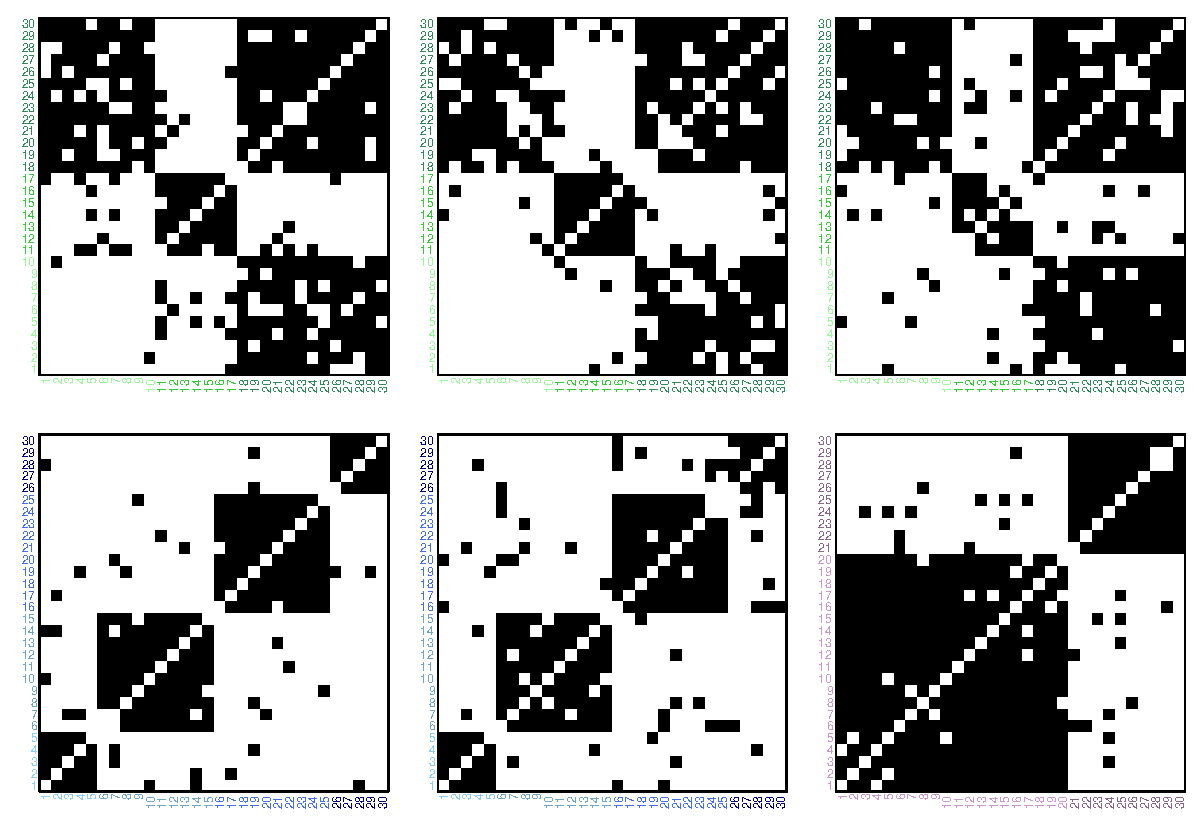
\includegraphics[width=0.41\textwidth]{Y30simShade.pdf}
\vspace{-0.2cm}
\mycaption{Adjacency matrices for simulated data set of 30 nodes with 6 layers of observations. The colors green, blue and purple represent the clustering of the layers.}
\end{center}

\vspace{0.5cm}

%%% RASHAD Model
\begin{center}
  \pbox{0.8\columnwidth}{}{linewidth=1.5mm,framearc=0.1,linecolor=lightblue,fillstyle=gradient,
    gradangle=0,gradbegin=white,gradend=whiteblue,gradmidpoint=2.0,framesep=0.7em}{
    \begin{center}
      {\large \bf RASHAD Model}
    \end{center}
  }
\end{center}

\vspace{1cm}
 
Let $A_1, \ldots, A_N$ be the sequence of binary adjacency matrices representing the multilayer undirected network data set with no self-edges. 

\vspace{.2cm}

\begin{itemize}
\item Each layer $i=1, \ldots,N$ consists of a $V \times V$ symmetric matrix $A_i$ such that $A_{i[v,u]}=A_{i[u,v]}  =1$ if there is a connection between nodes $v$ and $u$ in layer $i$, and $0$ otherwise. 

\vspace{.2cm}

\item The cluster assignments $c_1,\ldots,c_N$ with $c_i \in \{1, \ldots,  K\}$ indicate the color of layer $i$. 

\vspace{.2cm}

\item The color-specific partition of the node set is obtained via $s_{1k}, \ldots, s_{Vk}$, with $s_{vk} \in  \{1, \ldots,  H_k\}$ the shade of node $v$ in color $k$ and $H_k$ the total number of communities in color $k$.
\end{itemize}

\vspace{0.5cm}

This construction leads to the following generative mechanism:
\begin{eqnarray}
A_{i[v,u]}=A_{i[u,v]} \mid c_i=k &\sim& \mbox{Bern}(\pi_{k[v,u]}),\label{eq_1} \\
\pi_{k[v,u]} \mid s_{vk}=h, s_{uk}=h'&=&\theta_{k[h,h']}.
\label{eq_2}
\end{eqnarray}


%The  joint probability for the multilayer network data $A_1, \ldots, A_N$ is
%\begin{eqnarray*}
%\mbox{pr}\{A_{1},\ldots, A_{N} \mid- \}&{=}&\prod_{k=1}^K \prod_{h=1}^{H_k} \prod_{h'=1}^{h} \theta_{k[h,h']}^{n_{k[h,h']}}(1-\theta_{k[h,h']})^{\bar{n}_{k[h,h']}},
%\label{eq_mod}
%\end{eqnarray*}
%where $n_{k[h,h']}$ and $\bar{n}_{k[h,h']}$ are the total number of observed edges and non-edges.

\vspace{0.2cm}

\begin{center}
\textbf{Prior Specification}
\end{center}

\begin{itemize}
 \item The prior on interaction probabilities is:
 $ \theta_{k[h,h']} \stackrel{{\small{\mbox{iid}}}}{\sim} \mbox{Beta}(a,b)$

 \vspace{.2cm}

 \item Chinese Restaurant Processes (CRP) for the cluster assignments at both levels allows the number of clusters to be random:
 \begin{align*}
c=(c_1,\ldots,c_N) \sim \mbox{CRP}(\alpha_c),\\
s_{k}=(s_{1k}, \ldots, s_{Vk})\sim \mbox{CRP}(\alpha_k).
\end{align*}
The prior distribution over colors for the $i$th layer, conditioned on the colors of the others $c_1,\ldots ,c_{i-1},c_{i+1}, \ldots, c_{N}$ is
\begin{eqnarray*}
\mbox{pr}(c_i=k \mid \ldots) = \begin{cases} \frac{n_{k,-i}}{N-1+\alpha_c} & \quad \text{for} \ \ k=1, \ldots, K_{-i}, \\ \frac{\alpha_c}{N-1+\alpha_c} & \quad \text{for} \ \ k=K_{-i}+1,\\ \end{cases} 
\end{eqnarray*}
where $n_{k,-i} $ is the total number of layers associated to color $k$. 

\vspace{.2cm}

Similarly, for the shading mechanism:
\begin{eqnarray*}
\mbox{pr}(s_{vk}=h \mid \ldots) = \begin{cases} \frac{m_{hk,-v}}{V-1+\alpha_k} & \quad \text{for} \ \ h=1, \ldots, H_{k,-v}, \\ \frac{\alpha_k}{V-1+\alpha_k} & \quad \text{for} \ \  h=H_{k,-v}+1,\\ \end{cases} 
 \label{shade}
\end{eqnarray*}
independently, for each $k=1, \ldots, K$, where $m_{hk,-v}$ denotes the total number of nodes with shade $h$ of color $k$, when node $v$ is held out.
\item Gamma hyperpriors on $\alpha_c$ and $\alpha_k$.
\end{itemize}

Posterior samples are obtained via collapsed Gibbs sampler marginalizing over the interaction probabilities and results of Escobar and West (1995).

\vspace{.25cm}\begin{center}\pbox{0.8\columnwidth}{}{linewidth=1.5mm,framearc=0.1,linecolor=lightblue,
fillstyle=gradient,gradangle=0,gradbegin=white,gradend=whiteblue,gradmidpoint=1.0,framesep=0.7em}
{\begin{center}{\large \bf Application}\end{center}}\end{center}
\vspace{.1cm}

\begin{itemize}
\item We use real data from an Indian village in the state of Karnataka. 
\item Six types of relationships (layers)
between the 114 households (nodes) of the village.
\item Sparse networks with an average percent of links of 2.4\% except for
the temple relationship with only 0.25\%.
\item The model identifies attending the same temple as the only relationship with
different community structure across households. 
%\item The largest community consists of 
%94 households with no temple links within or between.
%\item The other relationships display 12 communities of households. The largest community 
%consists of 43 households with no interactions within and very few interactions with other communities.
\end{itemize}

\begin{center}
\includegraphics[width=0.45\textwidth]{pairxiKar6.pdf}
\vspace{-0.7cm}
\mycaption{Mean posterior pairwise incidence matrices for layers of Karnataka village. Red represents a high probability of two households to have the same shade of color within each layer.}
\end{center}

%%% Discussion and Future Work
\begin{center}\pbox{0.8\columnwidth}{}{linewidth=1.5mm,framearc=0.1,linecolor=lightblue,fillstyle=gradient,gradangle=0,
gradbegin=white,gradend=whiteblue,gradmidpoint=1.0,framesep=0.7em}{\begin{center}{\large \bf Discussion}\end{center}}\end{center}
\vspace{.1cm}

\begin{itemize}
\item We developed an efficient algorithm which allows automatic learning of the total number of clusters at the layer and nodes levels.
\item RASHAD can easily accommodate other type of data and priors for random partitions such as Pitman-Yor process.
\end{itemize}

{\small{\bf Acknowledgements:} Participation in this conference was supported in part by the WiML travel grant. This work is supported by the Foester-Bernstein Postdoctoral Fellowship.}

%%% Discussion and Future Work
%\vspace{.25cm}\begin{center}\pbox{0.8\columnwidth}{}{linewidth=2mm,framearc=0.1,linecolor=lightblue,
%fillstyle=gradient,gradangle=0,gradbegin=white,gradend=whiteblue,gradmidpoint=1.0,framesep=1em}
%{\begin{center}{\large \bf Application to NLTCS}\end{center}}\end{center}\vspace{.65cm}
%
%NLTCS: survey about health/functional status of Americans $65^{+}$ (appx 20,000 individuals/ wave).
%\begin{itemize}
%%\item Approximately 20,000 individuals/wave.
%%who were tracked/surveyed at five-year intervals.  
%%\item At each wave, some individuals have died and were replaced.
%%\vspace*{0.4em}
%%thus the files contain overlapping but different sets of individuals. 
%\item Test the record matching on three of the six waves.
%\item Data used here: DOB, sex, state, and office location, (and unique ID). 
%\end{itemize}
%
%\vspace*{0.5em}


%\begin{minipage}[c]{0.49\linewidth}
%\begin{center}
%\includegraphics[scale=0.55]{pics/roc_both.ps}
%\end{center}
%\end{minipage}
%\begin{minipage}[c]{0.49\linewidth}
%\mycaption{ We plot both ROC curves under SMERE and SMERED for the most probable MMSs and compare them to the simple baseline of exact matching (triangle). 
%}
%\end{minipage}
%
%\begin{itemize}
%\item For the same FNR,
%the FPR  is higher under SMERED than under SMERE. 
%%\item This is again due to problems in linkage using SMERED when the categorical information is very limited. When the FNR is small, performance is very similar under SMERE and SMERED. 
%\item The baseline can \emph{never change}, whereas, under our algorithm we can relax the FPR or FNR for performance. The ``near-twins" baseline does not appear on this plot since its FPR is 12.61.
%\end{itemize}
%
%\vspace{3em}
%
%
%\begin{minipage}[c]{0.49\linewidth}
%\begin{center}
%\includegraphics[scale=0.8]{pics/network_curves_center.ps}
%\end{center}
%\end{minipage}
%\begin{minipage}[c]{0.49\linewidth}
%\mycaption{ Each node is a record and edges are drawn between records with shared most probable MMSs. Color indicates whether or not the probability of the shared most probable MMS was above (green) or below (red) a threshold of 0.8. The curvy edges indicate that SMERED and the NLTCS do not agree on the linkage. The straight edges indicate linkage agreement. }
%\end{minipage}
%\vspace*{0.5em}


%\begin{minipage}[c]{0.49\linewidth}
%\begin{center}
%\includegraphics[scale=0.55]{pics/posterior_full_run_nostates_heatmaprun2.ps}
%\end{center}
%\end{minipage}
%\begin{minipage}[c]{0.49\linewidth}
%\mycaption{Estimate of posterior density of unknown population size. Under ground truth is known to be 34,945.}
%\end{minipage}
%\vspace*{0.5em}

%Calculate posterior matching probabilities (preserving transitivity), for any record of interest. 
%\begin{itemize}
% \item Suppose we are interested in record 10084, what records are potential matches (and associated probabilities). 
%\item Find that records 5583, 10084, and 6131 are all the same latent individual (with the same set of field values). 
%\end{itemize}
%
%\begin{center}
%\begin{tabular}{c|ccc}
%sets of records & 
% 1.10084       &        3.5583; 1.10084  &    3.5583; 1.10084; 2.6131  \\ \hline
%posterior probability & 0.001 & 0.004  & 0.995\\
%\end{tabular}
%\end{center}



%\vspace{.25cm}\begin{center}\pbox{0.8\columnwidth}{}{linewidth=2mm,framearc=0.1,linecolor=lightblue,
%fillstyle=gradient,gradangle=0,gradbegin=white,gradend=whiteblue,gradmidpoint=1.0,framesep=1em}
%{\begin{center}{\large \bf Simulation Studies}\end{center}}\end{center}\vspace{.3cm}
%\vspace*{1em}
%
%We simulate data from the NLTCS based on the proposed model with varying levels of distortion (none, 0.25\%, 0.5\%, 1\%, 2\%, 5\%). 
%\begin{itemize}
%\item 
%\item  Use our MCMC algorithm to assess how well we can match under ``noisy data."
%\end{itemize}
%
%\vspace*{-5em}
%\begin{center}
%\includegraphics[scale=0.65]{pics/distortion_rates_all.ps}
%\includegraphics[scale=0.65]{pics/distortion_six.ps}
%\mycaption{(Left): FNR and FPR versus distortion.
%(Right): Posterior density estimates for 6 levels of distortion and ground truth (red). As distortion increases (and approaches 2\% per field), we undermatch the true population size, however as distortion increases to high levels (5\%), the model overmatches. We expect continued overmatching at higher levels of distortion.}
%\end{center}
%

%%%
%%%% Discussion and Future Work
%\vspace{.25cm}\begin{center}\pbox{0.8\columnwidth}{}{linewidth=2mm,framearc=0.1,linecolor=lightblue,
%fillstyle=gradient,gradangle=0,gradbegin=white,gradend=whiteblue,gradmidpoint=1.0,framesep=1em}
%{\begin{center}{\large \bf  Ongoing Work}\end{center}}\end{center}\vspace{.3cm}
%\begin{itemize}
%%\item Record linkage for $k$ files $\rightarrow$ many challenges. 
%%\item Novel work with $k$ files: representation of linkage structure and flexibility for estimation/error rates and dealing with HD parameter space.
%\item Clusters records to latent individuals using an EB approach. 
%\item Incorporates both categorical and string data.
%%\item The probability of observing a given word is $\propto$ the empirical frequency of the word times $c.$
%% \item $c$ shrinks exponentially in the distance from the true value.
%\[
%\Pr(\text{observe string }w^{\prime} \mid \text{true string }w) \propto \Pr_{\text{empirical}}(w^{\prime})\;e^{-c\,d(w^{\prime},w)}.
%\]
%\item The string metric $d$ is general and decided by the user. % Can be validated using traditional methods.
%
%\end{itemize}
%\vspace{1cm}
%
%
%%\vspace{1cm}
%\begin{minipage}[H]{0.45\linewidth}
%\centering
%\includegraphics[scale=0.7]{pics/posterior_5000_v5_distort_1percent.ps}
%\mycaption{Posterior density for N in simulation study. The FNR and FPR:  0.04 and  0.02. 
%%The posterior mean and standard error are 473 and 10.  
%%The code used to produce this plot was $\texttt{RL\_gibbs-20140120\_v6.R}$. The total run time is 2.5 hours. 
%}
%\label{fig:figure1}
%\end{minipage}
%\hspace{0.5cm}
%\begin{minipage}[H]{0.45\linewidth}
%\centering
%\includegraphics[scale=0.7]{pics/network_EB_5000_v5_1percent_distortion.ps}
%\mycaption{Shared MPMMS graphical representation of simulation study.  Only makes one false positive set.
%% The algorithm only makes one false positive set consistent with the FPR being 0.02.
%% The code used to produce this plot was $\texttt{RL\_gibbs-20140120\_v6.R}$.
%}
%\label{fig:figure2}
%\end{minipage}
%
%\vspace*{1em}

%{\bf \underline{Acknowledgements:}}\\
%{\bf This work was supported by NSF Grant SES 1130706. The views expressed here are 
%those of the authors and do not reflect those of the NSF or U.S. Census Bureau. 
%}\\

%\vspace*{-3em}
%\tiny{
%%\scriptsize{
%\bibliographystyle{unsrt}
%\bibliography{references}
%}
\phantom{.}
\end{multicols}



\end{poster}

\end{document}

% \includegraphics{plots/band1.eps}
%      \includegraphics{plots/band2.eps}
%      \includegraphics{plots/band3.eps}\\
%      \includegraphics{plots/band4.eps}
%      \includegraphics{plots/band5.eps}
%      \includegraphics{plots/band6.eps}\\
%      \includegraphics{plots/band7.eps}
%      \includegraphics{plots/band8.eps}\\
%      \includegraphics{plots/legend1.eps}
%      \mycaption{Medians (smooth lines) and $95\%$ probability bands (shaded regions around the medians) of the posterior distributions of the main effects of the LCM at 8 different MODIS bands.}
      


